


%Translate this Latex book chapter to Spanish. Output in Latex format. Rearrange bullet points (\items) into full paragraphs. Make sure that sentences are connected in a more fluid way as they come.

\begin{itemize}
\item Las redes neuronales son una familia muy popular de modelos de aprendizaje automático formados por unidades llamadas \textbf{neuronas}.
\item Una neurona es una unidad computacional que tiene entradas y salidas escalares.
\item Cada entrada tiene asociado un peso $w$.
\item La neurona multiplica cada entrada por su peso y luego los suma (también son posibles otras funciones como \textbf{max}).
\item Aplica una función de activación $g$ (generalmente no lineal) al resultado y lo pasa a su salida.
\item Se pueden apilar múltiples capas.
\item La función de activación no lineal $g$ juega un papel crucial en la capacidad de la red para representar funciones complejas.
\item Sin la no linealidad en $g$, la red neuronal solo puede representar transformaciones lineales de la entrada.
\end{itemize}

Ejemplo: Red feedforward con dos capas

\begin{figure}[htb]
	\centering
	 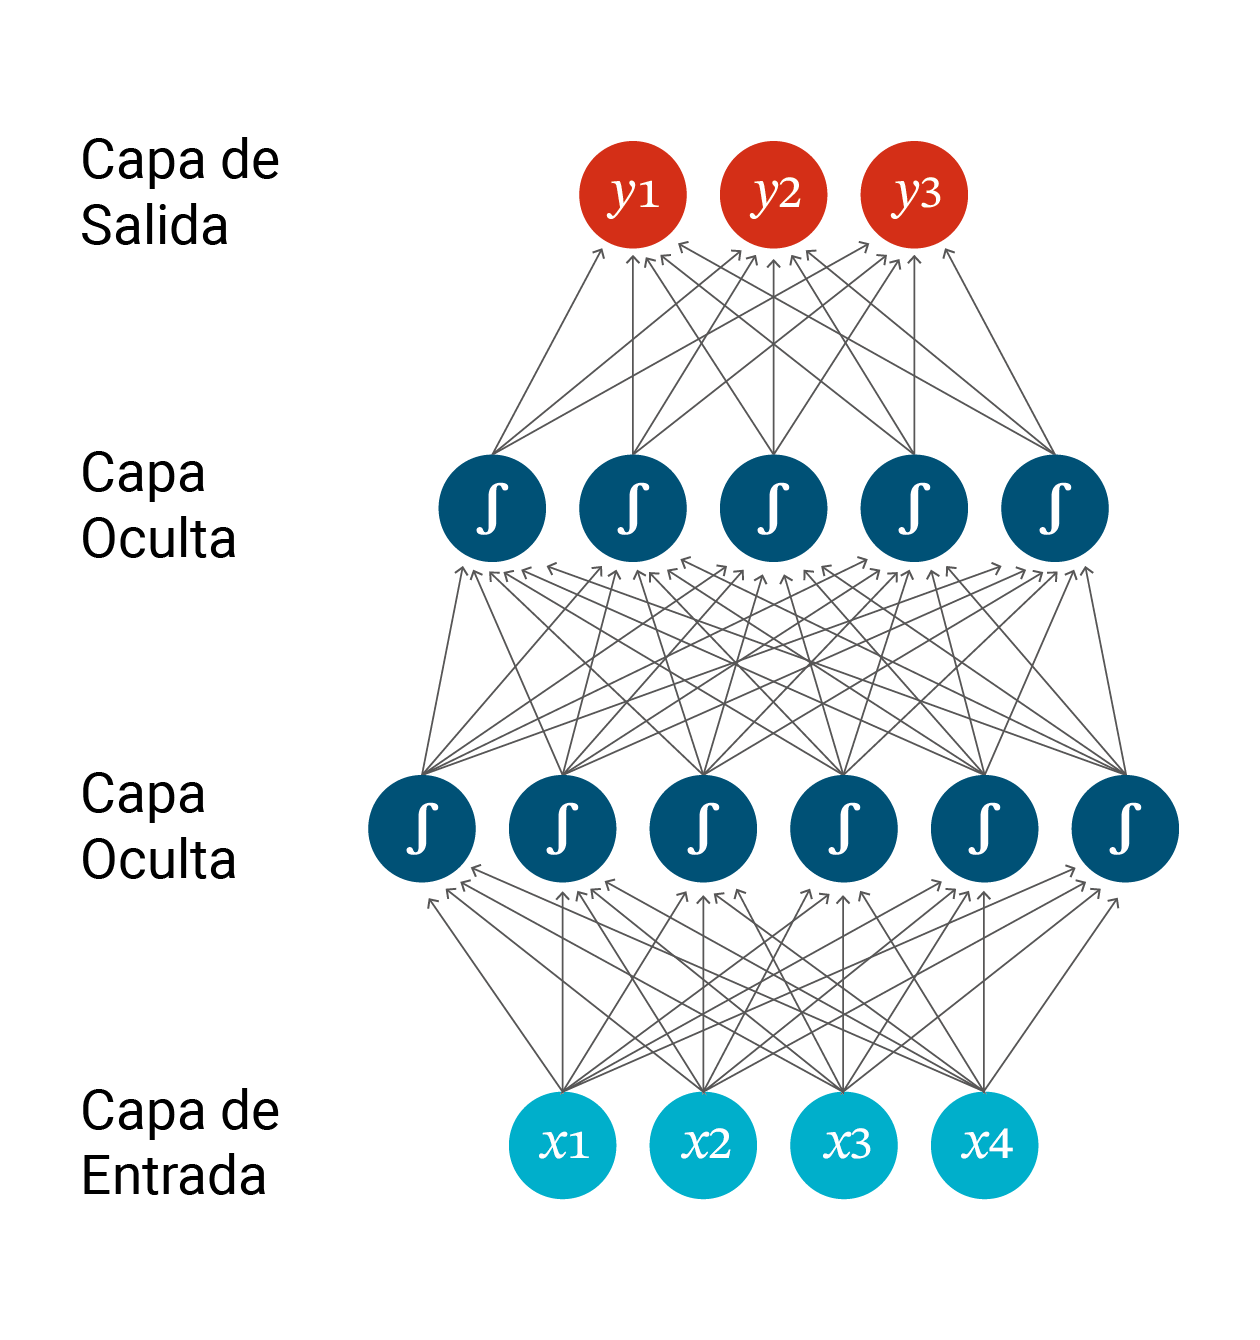
\includegraphics[scale=0.38]{pics/NN-example.png}
\end{figure}

\footnotetext{Fuente:\cite{goldberg2017neural}}

\section{Redes neuronales feedforward}

\begin{itemize}
\item La red feedforward de la imagen es una concatenación de modelos lineales separados por funciones no lineales.
\item Los valores de cada fila de neuronas en la red se pueden pensar como un vector.
\item La capa de entrada es un vector de 4 dimensiones $(\vec{x})$, y la capa superior es un vector de 6 dimensiones $(\vec{h}^1)$.
\item La capa completamente conectada se puede pensar como una transformación lineal de 4 dimensiones a 6 dimensiones.
\item Una capa completamente conectada implementa una multiplicación de vector-matriz, $\vec{h}=\vec{x}W$.
\item El peso de la conexión desde la neurona $i$-ésima en la fila de entrada hasta la neurona $j$-ésima en la fila de salida es $W_{[i,j]}$.
\item Los valores de $\vec{h}$ se transforman mediante una función no lineal $g$ que se aplica a cada valor antes de pasar al siguiente nivel.

\end{itemize}

\footnotetext{Se asume que los vectores son vectores fila y los índices en superíndices corresponden a las capas de la red.}

\paragraph{Capas completamente conectadas como multiplicaciones de vectores y matrices}
\begin{figure}[htb]
	\centering
	 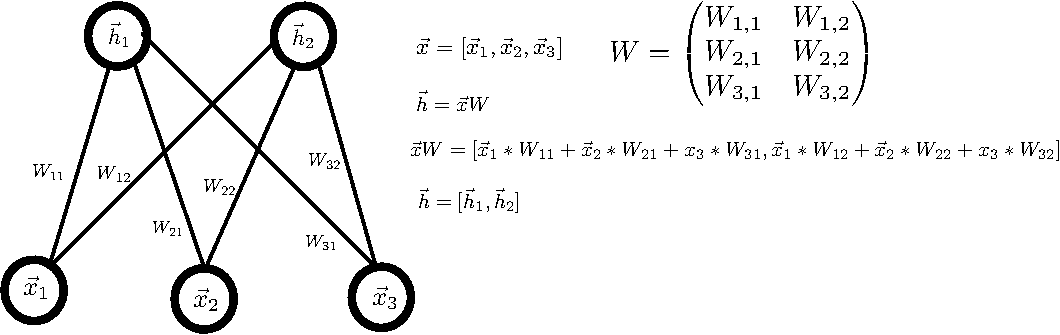
\includegraphics[scale=0.65]{pics/neural_net_mat_mul.pdf}
\end{figure}

\subsection{Redes neuronales como funciones matemáticas}

\begin{itemize}
\item El Perceptrón Multicapa (MLP, por sus siglas en inglés) de la figura se llama MLP2 porque tiene dos capas ocultas.
\item Un modelo más simple sería MLP1, un perceptrón multicapa de una capa oculta:
\begin{center}
\begin{equation}
\begin{split}
\vec{\hat{y}} = NN_{MLP1}(\vec{x}) = g(\vec{x}W^{1}+\vec{b}^{1})W^{2}+\vec{b}^{2} \\
\vec{x} \in \mathcal{R}^{in}, W^{1} \in \mathcal{R}^{d_{in}\times d_{1}}, \vec{b}^{1} \in \mathcal{R}^{d_{1}}, W^{2} \in \mathcal{R}^{d_{1}\times d_{out}}, \vec{b}^{2} \in \mathcal{R}^{d_{out}}, \vec{\hat{y}} \in \mathcal{R}^{d_{out}}
\end{split}
\end{equation}
\end{center}

\item Aquí, $W^{1}$ y $\vec{b}^{1}$ son una matriz y un término de sesgo para la primera transformación lineal de la entrada.
\item La función $g$ es una función no lineal que se aplica elemento a elemento (también se llama no linealidad o función de activación).
\item $W^{2}$ y $\vec{b}^{2}$ son la matriz y el término de sesgo para una segunda transformación lineal.

\item Al describir una red neuronal, se deben especificar las dimensiones de las capas ($d_{1}$), la entrada ($d_{in}$) y la salida ($d_{out}$).
\item MLP2 se puede escribir como la siguiente función matemática:
\begin{center}
\begin{equation}
\begin{split}
NN_{MLP2}(\vec{x}) & =  \vec{\hat{y}}  \\
\vec{h}^{1} &  = \vec{x}W^{1}+\vec{b}^{1} \\
\vec{h}^{2} &  = g^{1}(\vec{h}^{1})W^{2}+\vec{b}^{2} \\
\vec{y} &  = g^{2}(\vec{h}^{2})W^{3}\\
\vec{y} &  = (g^2(g^1(\vec{x}W^{1}+\vec{b}^{1})W^2+\vec{b}^2))W^3.\\
\end{split}
\end{equation}
\end{center}
\item Las matrices y los términos de sesgo que definen las transformaciones lineales son los parámetros de la red.
\item Al igual que en los modelos lineales, es común referirse a la colección de todos los parámetros como $\Theta$.
\end{itemize}

\section{Capacidad de representación}

\begin{itemize}
\item \cite{hornik1989multilayer} y \cite{cybenko1989approximation} mostraron que un perceptrón multicapa de una capa oculta (MLP1) es un aproximador universal.
\item MLP1 puede aproximar todas las funciones continuas en un subconjunto cerrado y acotado de $\mathcal{R}^n$.
\item Esto puede sugerir que no hay razón para ir más allá de MLP1 en arquitecturas más complejas.
\item El resultado no dice qué tan fácil o difícil es establecer los parámetros basándose en los datos de entrenamiento y un algoritmo de aprendizaje específico.
\item Tampoco garantiza que un algoritmo de entrenamiento encontrará la función correcta que genera nuestros

datos de entrenamiento.
\item Finalmente, no establece qué tan grande debería ser la capa oculta.
\item En la práctica, entrenamos redes neuronales con cantidades relativamente pequeñas de datos utilizando métodos de búsqueda local.
\item También utilizamos capas ocultas de tamaños relativamente modestos (hasta varios miles).
\item El teorema de aproximación universal no ofrece ninguna garantía bajo estas condiciones.
\item Sin embargo, definitivamente hay beneficios en probar arquitecturas más complejas que MLP1.
\item En muchos casos, sin embargo, MLP1 brinda resultados sólidos.
\end{itemize}

\section{Funciones de activación}
\begin{itemize}
\item La no linealidad $g$ puede tomar muchas formas.
\item Actualmente no existe una buena teoría sobre qué no linealidad aplicar en qué condiciones.
\item Elegir la no linealidad correcta para una tarea determinada es en su mayor parte una cuestión empírica.
\end{itemize}

\paragraph{Sigmoide}
\begin{itemize}
\item La función de activación sigmoide $\sigma(x) = \frac{1}{1+e^{-x}}$ es una función en forma de S, que transforma cada valor x en el rango $[0, 1]$.
\item El sigmoide fue la no linealidad canónica para las redes neuronales desde su inicio.
\item Actualmente se considera obsoleta para su uso en capas internas de redes neuronales, ya que las opciones que se enumeran a continuación funcionan mucho mejor empíricamente.
\end{itemize}

\begin{figure}[htb]
	\centering
	 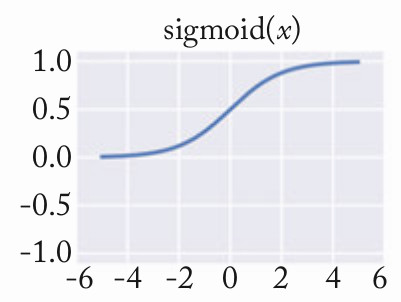
\includegraphics[scale=0.3]{pics/sigmoid2.png}
\end{figure}

\paragraph{Tangente hiperbólica (tanh)}
\begin{itemize}
\item La función de activación tangente hiperbólica $\operatorname{tanh}(x) = \frac{e^{2x}-1}{e^{2x}+1}$ es una función en forma de S que transforma los valores x en el rango $[-1, 1]$.
\end{itemize}

\begin{figure}[htb]
	\centering
	 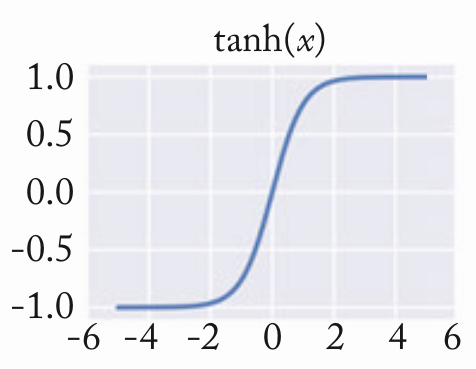
\includegraphics[scale=0.3]{pics/tanh.png}
\end{figure}

\paragraph{Hard tanh}
\begin{itemize}
\item La función de activación hard-tanh es una aproximación de la función tangente hiperbólica que es más rápida de calcular y encontrar sus derivadas:
\end{itemize}

  \[
    \operatorname{hardtanh}(x) = \left\{\begin{array}{lr}
        -1 & x < -1\\
        1 & x > 1\\
        x & \text{en otros casos.}
        \end{array} \right\}
  \]

\begin{figure}[htb]
	\centering
	 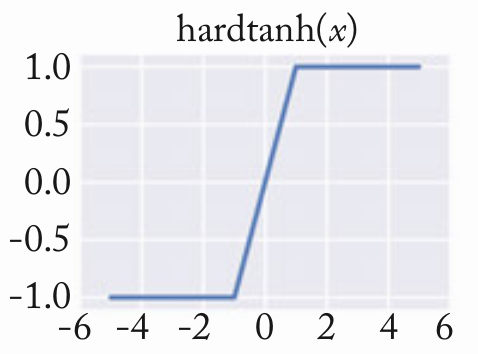
\includegraphics[scale=0.3]{pics/hardtanh.png}
\end{figure}

\paragraph{ReLU}
\begin{itemize}
\item La función de activación rectificador \cite{glorot2011deep}, también conocida como unidad lineal rectificada, es una función de activación muy simple.
\item Es fácil de trabajar y se ha demostrado muchas veces que produce excelentes resultados.
\item La

función ReLU se define como $ReLU(x) = \max(0, x)$.
\end{itemize}

\begin{figure}[htb]
	\centering
	 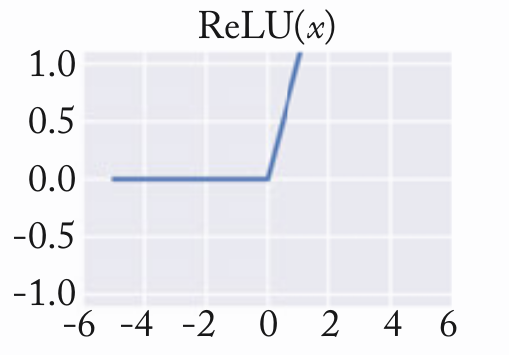
\includegraphics[scale=0.3]{pics/relu.png}
\end{figure}

\paragraph{Leaky ReLU}
\begin{itemize}
\item La función Leaky ReLU es similar a ReLU, pero permite una pequeña pendiente para valores negativos.
\item Se define como $LeakyReLU(x) = \max(\alpha x, x)$, donde $\alpha$ es un hiperparámetro pequeño (por lo general, en el rango de $0.01$ a $0.2$).
\end{itemize}

%\begin{figure}[htb]
%	\centering
%	 \includegraphics[scale=0.3]{pics/leakyrelu.png}
%\end{figure}

\paragraph{ELU}
\begin{itemize}
\item La función de activación ELU (Exponential Linear Unit) \cite{clevert2015fast} es una versión mejorada de ReLU que también tiene una pendiente para valores negativos.
\item Se define como $ELU(x) = \left\{\begin{array}{lr}
        \alpha (e^x - 1) & x < 0\\
        x & \text{en otros casos.}
        \end{array} \right\}$
\item Aquí, $\alpha$ es un hiperparámetro que controla la pendiente negativa.
\end{itemize}

%\begin{figure}[htb]
%	\centering
%	 \includegraphics[scale=0.3]{pics/elu.png}
%\end{figure}

Estas son solo algunas de las muchas opciones disponibles para las funciones de activación en redes neuronales. La elección de la función de activación puede depender del problema específico y puede requerir pruebas empíricas para determinar cuál funciona mejor.



\subsection{Problemas Prácticos}
En términos generales, tanto las unidades ReLU como las unidades tangente hiperbólica (tanh) funcionan bien y superan significativamente a la función sigmoide. Sin embargo, puede ser beneficioso experimentar con ambas activaciones, ya que cada una puede funcionar mejor en diferentes configuraciones. La Figura 1 muestra las formas de las diferentes funciones de activación, junto con las formas de sus derivadas.

\begin{figure}[htb]
	\centering
	 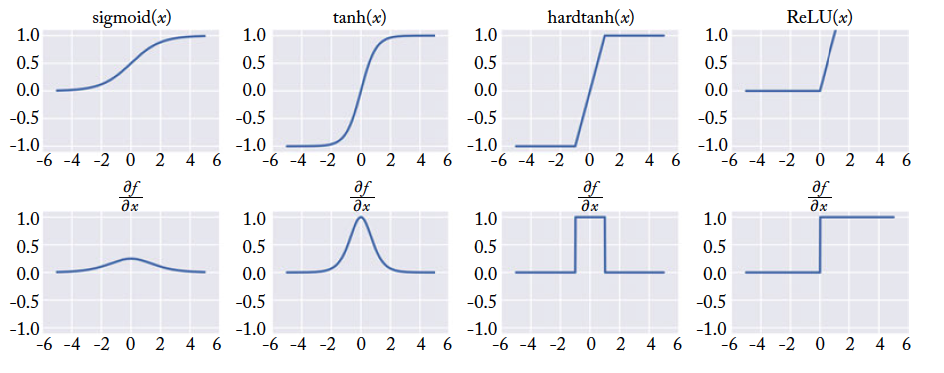
\includegraphics[scale=0.35]{pics/activations.png}
\end{figure}

\footnotetext{Fuente:\cite{goldberg2017neural}}

\section{Capas de Embedding}
En el procesamiento del lenguaje natural (PLN), la entrada a la red neuronal contiene características categóricas simbólicas (por ejemplo, palabras de un vocabulario cerrado, n-gramas de caracteres, etiquetas POS). En los modelos lineales, generalmente representamos la entrada con vectores dispersos, como la suma, el promedio o la concatenación de vectores codificados one-hot (la suma o el promedio pueden producir una representación de bolsa de palabras). En las redes neuronales, es común asociar cada valor de característica posible (es decir, cada palabra en el vocabulario, cada categoría de etiqueta POS) con un vector denso de $d$ dimensiones.

Estos vectores luego se consideran parámetros del modelo y se entrenan conjuntamente con los demás parámetros. El mapeo desde valores de características simbólicas, como "número de palabra 1249", a vectores de $d$ dimensiones se realiza mediante una capa de embedding (también llamada capa de búsqueda). Los parámetros en una capa de embedding de palabras son simplemente una matriz $E \in \mathbb{R}^{|vocab|\times d}$ donde cada fila corresponde a una palabra diferente en el vocabulario. La operación de búsqueda es simplemente una indexación: $v_{1249} = E_{[1249,:]}$. Si la característica simbólica se codifica como un vector one-hot $\vec{x}$, la operación de búsqueda se puede implementar como una multiplicación de matriz-vector $\vec{x}E$. Los vectores de embedding se combinan antes de pasar a la siguiente capa. Las operaciones comunes de combinación son concatenación, suma y promedio. Una matriz de embeddings de palabras $E$ se puede inicializar con vectores de palabras preentrenados a partir de documentos no etiquetados utilizando métodos específicos basados en la hipótesis distribucional, como los implementados en Word2Vec (que se discutirán más adelante en el curso).

\begin{figure}[htb]
	\centering
	 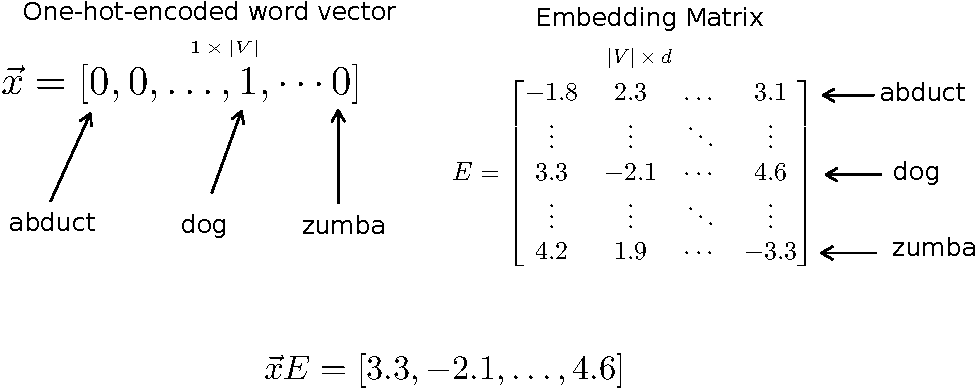
\includegraphics[scale=0.65]{pics/emb_matrix.pdf}
\end{figure}

\subsection{Vectores Densos vs Representaciones One-hot}
¿Cuáles son los beneficios de representar nuestras características como vectores en lugar de como identificadores únicos? ¿Deberíamos siempre representar las características como vectores densos? Consideremos los dos tipos de representaciones.

\begin{enumerate}
 \item \textbf{One Hot}: cada característica es su propia dimensión.
 \begin{itemize}
  \item La dimensionalidad del vector one-hot es igual al número de características distintas.
  \item  Las características son completamente independientes entre sí. La característica "la palabra es 'perro'" es tan diferente de "la palabra es 'pensando'" como lo es de "la palabra es 'gato'".
 \end{itemize}
\item \textbf{Dense}: cada característica es un vector de d dimensiones.
\begin{itemize}
 \item La dimensionalidad del vector es d.
 \item El entrenamiento del modelo hará que características similares tengan vectores similares: la información se comparte entre características similares.
\end{itemize}
\end{enumerate}




\paragraph{Ejemplo: Vectores Densos vs Representaciones One-hot}

\begin{figure}[htb]
	\centering
	 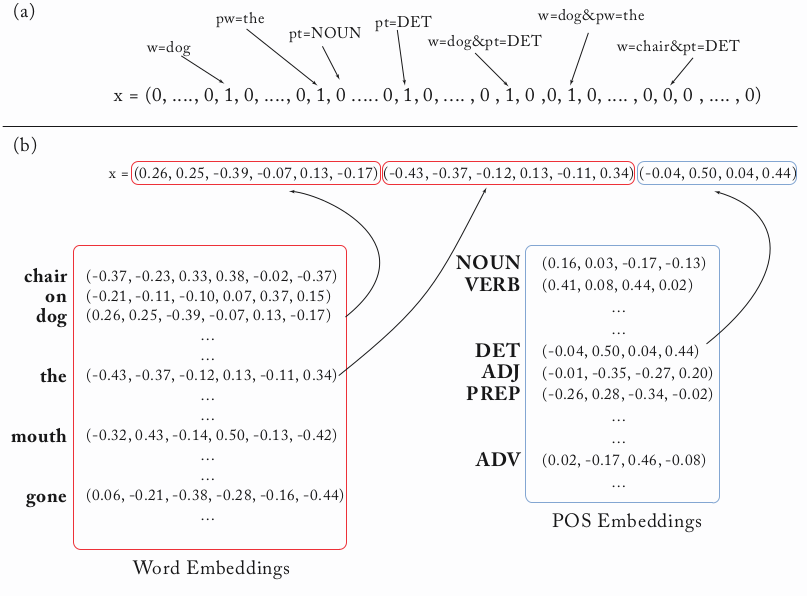
\includegraphics[scale=0.35]{pics/denseonehot.png}
\end{figure}

La figura anterior muestra dos codificaciones de la información: la palabra actual es "perro"; la palabra anterior es "el"; la etiqueta POS anterior es "DET".

(a) Vector de características dispersas:
\begin{itemize}
 \item Cada dimensión representa una característica.
\item Las combinaciones de características tienen sus propias dimensiones.
\item Los valores de las características son binarios.
\item La dimensionalidad es muy alta.
\end{itemize}


(b) Vector de características densas basado en embeddings.

\begin{itemize}
\item Cada característica principal se representa como un vector.
\item  Cada característica se corresponde con varias entradas del vector de entrada.
\item No hay una codificación explícita de combinaciones de características.
\item La dimensionalidad es baja.
\item Los mapeos de características a vectores provienen de una tabla de embeddings.
\end{itemize}


Un beneficio de usar vectores densos y de baja dimensionalidad es computacional: la mayoría de las bibliotecas de redes neuronales no funcionan bien con vectores dispersos de alta dimensionalidad. Sin embargo, este es solo un obstáculo técnico que se puede resolver con cierto esfuerzo de ingeniería.

El principal beneficio de las representaciones densas radica en el poder de generalización. Si creemos que algunas características pueden proporcionar pistas similares, vale la pena proporcionar una representación que pueda capturar estas similitudes. Supongamos que hemos observado la palabra "perro" muchas veces durante el entrenamiento, pero solo hemos observado la palabra "gato" unas pocas veces. Si cada una de las palabras se asocia con su propia dimensión (one-hot), las ocurrencias de "perro" no nos dirán nada sobre las ocurrencias de "gato". Sin embargo, en la representación de vectores densos, el vector aprendido para "perro" puede ser similar al vector aprendido para "gato". Esto permitirá que el modelo comparta fuerza estadística entre los dos eventos. Este argumento asume que hemos visto suficientes ocurrencias de la palabra "gato" como para que su vector sea similar al de "perro". Los vectores de palabras preentrenados (por ejemplo, Word2Vec, GloVe), que se discutirán más adelante en el curso, se pueden utilizar para obtener vectores densos a partir de texto no anotado.



\section{Entrenamiento de Redes Neuronales}

Las redes neuronales se entrenan de la misma manera que los modelos lineales. La salida de la red se utiliza para calcular una función de pérdida $L(\hat{y},y)$ que se minimiza en todos los ejemplos de entrenamiento utilizando descenso de gradiente. El algoritmo de retropropagación es una técnica eficiente para evaluar el gradiente de una función de pérdida $L$ en una red neuronal de alimentación directa con respecto a todos sus parámetros (Bishop, 2006). Los parámetros de la red incluyen $W^1, \vec{b}^1, \dots, W^m, \vec{b}^m$ para una red de $m$ capas. Cabe destacar que los superíndices se utilizan para denotar los índices de las capas (no exponenciación). Para simplificar, asumiremos que $L$ se calcula sobre un solo ejemplo. El desafío radica en que en las redes neuronales el número de parámetros puede ser enorme y necesitamos una forma eficiente de calcular los gradientes. La idea es aplicar la regla de la cadena de derivadas de manera inteligente.

\begin{figure}[htb]
	\centering
	 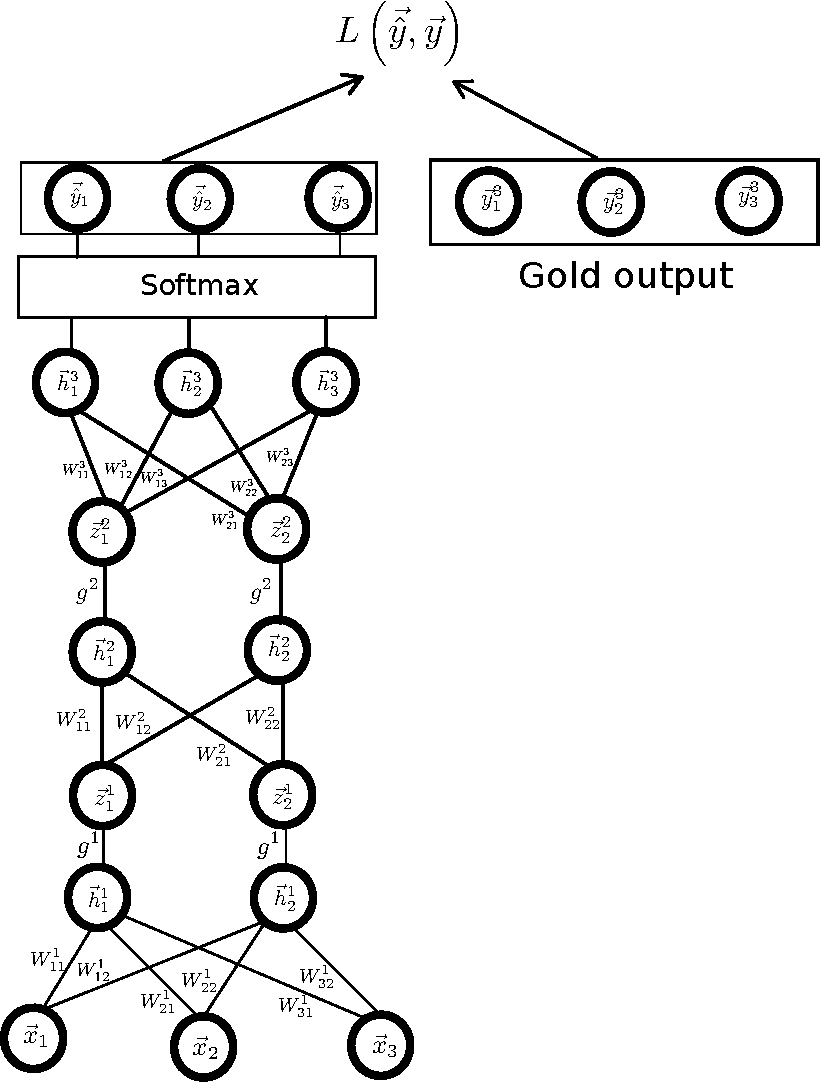
\includegraphics[scale=0.41]{pics/neural_net.pdf}
\end{figure}

\section{Recordatorio de la Regla de la Cadena en Derivadas}

La regla de la cadena simple establece que si $z = f(y)$ y $y = g(x)$, entonces

\begin{displaymath}
\frac{\partial z}{\partial x} = \frac{\partial z}{\partial y} \times \frac{\partial y}{\partial x}
\end{displaymath}

Por ejemplo, si $z= e^{y}$ y $y = 2x$, entonces

\begin{displaymath}
\frac{\partial z}{\partial x} = \frac{\partial z}{\partial y} \times \frac{\partial y}{\partial x} = e^{y} \times 2 = 2 e^{2x}
\end{displaymath}

\begin{figure}[htb]
	\centering
	 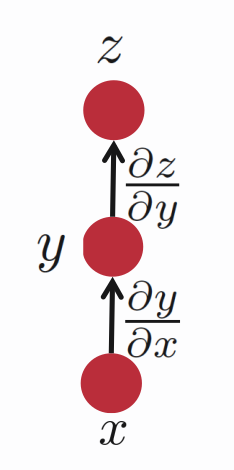
\includegraphics[scale=0.2]{pics/simple_chain_rule.png}
\end{figure}

La regla de la cadena múltiple establece que si $z = f(y_1,y_2)$, $y_1 = g_1(x)$ y $y_2 = g_2(x)$, entonces

\begin{displaymath}
\frac{\partial z}{\partial x} = \frac{\partial z}{\partial y_1} \times \frac{\partial y_1}{\partial x} + \frac{\partial z}{\partial y_2} \times \frac{\partial y_2}{\partial x}
\end{displaymath}

Por ejemplo, si $z= e^{y_1 \times y_2}$, $y_1 = 2x$ y $y_2 = x^2$, entonces

\begin{displaymath}
\frac{\partial z}{\partial x} = (e^{y_1 \times y_2}\times y_2) \times 2 + (e^{y_1 \times y_2}\times y_1) \times 2x = e^{2x^3} \times 6x^2
\end{displaymath}


\begin{figure}[htb]
	\centering
	 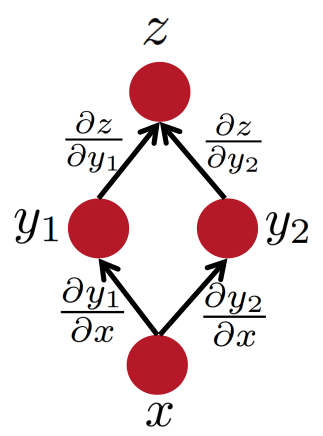
\includegraphics[scale=0.3]{pics/multiple_paths_chain_rule.png}
\end{figure}

La versión general de la regla de la cadena múltiple es:

\begin{displaymath}
 \frac{\partial z}{\partial x} = \sum_{i=1}^n \frac{\partial z}{\partial y_i} \times \frac{\partial y_i}{\partial x}
\end{displaymath}

\begin{figure}[htb]
	\centering
	 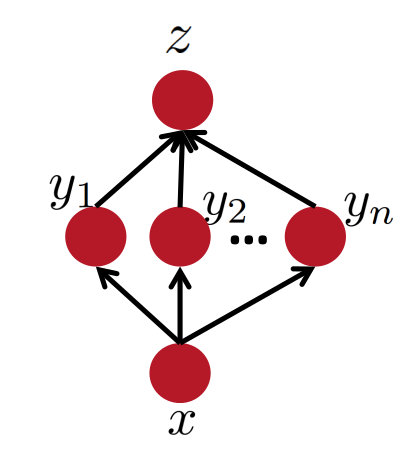
\includegraphics[scale=0.4]{pics/multiple_paths_chain_rule_general.png}
\end{figure}

\section{Retropropagación}

En una red de alimentación directa general, cada unidad calcula una suma ponderada de sus entradas de la siguiente forma:

\begin{equation}
\vec{h}_{[j]}^l = \left(\sum_{i}  W_{[i,j]}^l \times \vec{z}_{[i]}^{(l-1)}\right) + \vec{b}_{[j]}^l
\label{eq:sum}
\end{equation}

La variable $\vec{z}_{[i]}^{(l-1)}$ es una entrada que envía una conexión a la unidad $\vec{h}_{[j]}^l$, $W_{[i,j]}^l$ es el peso asociado con esa conexión, y $l$ es el índice de la capa.

Los vectores de sesgo $\vec{b}_{[j]}$ pueden excluirse de (eq. \ref{eq:sum}) e incluirse en la matriz de pesos $W_{[i,j]}^l$ al introducir una unidad adicional, o entrada, con una activación fija de +1.

Las entradas en la capa $l$, $\vec{z}_{[i]}^{(l-1)}$, son el resultado de aplicar la función de activación $g$ a las unidades de la capa anterior:

\begin{equation}
\vec{z}_{[j]}^{l} = g(\vec{h}_{[j]}^{l})
\label{eq:ac}
\end{equation}

Para la capa de entrada ($l=0$), $\vec{z}$ corresponde al vector de entrada $\vec{z} = \vec{x}$:

\begin{equation}
\vec{z}_{[j]}^0 = \vec{x}_{[j]}
\end{equation}

Para cada instancia en el conjunto de entrenamiento, proporcionamos el vector de entrada correspondiente $\vec{x}$ a la red. Luego calculamos las activaciones de todas las unidades ocultas y de salida en la red mediante la aplicación sucesiva de (eq. \ref{eq:sum}) y (eq. \ref{eq:ac}).

Este proceso a menudo se denomina propagación hacia adelante porque se puede considerar como un flujo de información hacia adelante a través de la red.

Ahora consideremos la evaluación de la derivada de $L$ con respecto a un peso $W_{[i,j]}^l$.

Suponiendo que la pérdida $L$ se calcula sobre un solo ejemplo, podemos observar que $L$ depende del peso $W_{[i,j]}^l$ únicamente a través de la suma de las entradas $\vec{h}_{[j]}^{l}$.

Por lo tanto, podemos aplicar la

regla de la cadena para derivadas parciales para obtener:

\begin{equation}
\frac{\partial L}{\partial W_{[i,j]}^l} = \frac{\partial L}{\partial \vec{h}_{[j]}^{l}} \times \frac{\partial \vec{h}_{[j]}^{l}}{\partial W_{[i,j]}^l}
\label{eq:chain}
\end{equation}

Ahora introducimos una notación útil:

\begin{equation}
\vec{\delta}_{[j]}^l \equiv \frac{\partial L}{\partial \vec{h}_{[j]}^l}
\label{eq:delta}
\end{equation}

Usando (\ref{eq:sum}), podemos escribir

\begin{equation}
\frac{\partial \vec{h}_{[j]}^l}{\partial W_{[i,j]}^l} = \vec{z}_{[i]}^{(l-1)}
\label{eq:part}
\end{equation}

Sustituyendo (\ref{eq:delta}) y (\ref{eq:part}) en (\ref{eq:chain}), obtenemos

\begin{equation}
\frac{\partial L}{\partial W_{[i,j]}^l} = \vec{\delta}_{[j]}^l \times \vec{z}_{[i]}^{(l-1)}
\label{eq:deltarule}
\end{equation}

La ecuación (\ref{eq:deltarule}) nos dice que la derivada requerida se obtiene simplemente multiplicando el valor de $\vec{\delta}_{[j]}^l$ por el valor de $\vec{z}_{[i]}^{(l-1)}$.

Por lo tanto, para evaluar las derivadas, solo necesitamos calcular el valor de $\vec{\delta}_{[j]}^l$ para cada unidad oculta y de salida en la red, y luego aplicar (\ref{eq:deltarule}) para actualizar los pesos de la red. Este proceso se conoce como retropropagación, ya que el cálculo del gradiente se propaga hacia atrás a través de la red.


Calcular $\vec{\delta}_{[j]}^m$ para las unidades de salida ($l=m$) suele ser directo, ya que las unidades de activación $\vec{h}_{[j]}^m$ se observan directamente en la expresión de pérdida.

Lo mismo se aplica a los modelos lineales poco profundos.

Para evaluar $\vec{\delta}_{[j]}^l$ para las unidades ocultas, nuevamente hacemos uso de la regla de la cadena para derivadas parciales:

\begin{equation}
\vec{\delta}_{[j]}^l \equiv \frac{\partial L}{\partial \vec{h}_{[j]}^l} = \sum_{k}\left( \frac{\partial L}{\partial \vec{h}_{[k]}^{l+1}} \times \frac{\partial \vec{h}_{[k]}^{l+1}}{\partial \vec{h}_{[j]}^l}\right)
\label{eq:deltachain}
\end{equation}

La suma se realiza sobre todas las unidades $\vec{h}_{[k]}^{l+1}$ a las que la unidad $\vec{h}_{[j]}^l$ envía conexiones.

Suponemos que las conexiones se realizan solo entre capas consecutivas en la red (desde la capa $l$ hasta la capa $(l+1)$).

Las unidades $\vec{h}_{[k]}^{l+1}$ podrían incluir otras unidades ocultas y/o unidades de salida.

Si ahora sustituimos la definición de $\vec{\delta}_{[j]}^l$ dada por la ecuación (\ref{eq:delta}) en la ecuación (\ref{eq:deltachain}), obtenemos:

\begin{equation}
\vec{\delta}_{[j]}^l \equiv \frac{\partial L}{\partial \vec{h}_{[j]}^l} = \sum_{k}\left( \vec{\delta}_{[k]}^{(l+1)}  \times \frac{\partial \vec{h}_{[k]}^{l+1}}{\partial \vec{h}_{[j]}^l} \right)
\label{eq:delta2}
\end{equation}

Ahora, para la expresión $\vec{h}_{[k]}^{l+1}$ podemos ir a su definición (ecuación \ref{eq:sum}):

\begin{displaymath}
\vec{h}_{[k]}^{(l+1)} = \left( \sum_{i} W_{[i,k]}^{l+1} \times \vec{z}_{[i]}^{l}\right) + \vec{b}_{[k]}^{(l+1)}
\end{displaymath}

Reemplazando ahora la ecuación (\ref{eq:ac}) $(\vec{z}_{[i]}^{l} = g(\vec{h}_{[i]}^{l}))$ en la ecuación anterior, obtenemos:

\begin{displaymath}
\vec{h}_{[k]}^{(l+1)} = \left( \sum_{i}   W_{[i,k]}^{l+1} \times g(\vec{h}_{[i]}^{l})\right)  + \vec{b}_{[k]}^{(l+1)}
\end{displaymath}

Al calcular $\frac{\partial \vec{h}_{[k]}^{l+1}}{\partial \vec{h}_{[j]}^l}$, todos los términos en la suma donde $i \neq j$ se cancelan.

Por lo tanto, tenemos:

\begin{equation}
\frac{\partial \vec{h}_{[k]}^{l+1}}{\partial \vec{h}_{[j]}^l} =  W_{[j,k]}^{l+1} \times g'(\vec{h}_{[j]}^{l})
\label{eq:partialhh}
\end{equation}

Sustituyendo la ecuación (\ref{eq:partialhh}) en la ecuación (\ref{eq:delta2}), obtenemos:

\begin{equation}
\vec{\delta}_{[j]}^l \equiv \frac{\partial L}{\partial \vec{h}_{[j]}^l} = \sum_{k} \left( \vec{\delta}_{[k]}^{(l+1)}  \times W_{[j,k]}^{l+1} \times g'(\vec{h}_{[j]}^{l}) \right)
\label{eq:delta3}
\end{equation}

Dado que $g'(\vec{h}_{[j]}^{l})$ no depende de $k$, podemos obtener la siguiente fórmula de retropropagación:

\begin{equation}
\vec{\delta}_{[j]}^l = g'(\vec{h}_{[j]}^{l}) \times \sum_{k} \left( \vec{\delta}_{[k]}^{(l+1)}  \times W_{[j,k]}^{l+1}\right)
\label{eq:delta4}
\end{equation}

Esto nos dice que el valor de $\vec{\delta}$ para una unidad oculta en particular se puede obtener propagando los $\vec{\delta}$ hacia atrás desde las unidades superiores en la red \cite{bishop2006pattern}.

El procedimiento de retropropagación se puede resumir de la siguiente manera:

\begin{enumerate}
  \item Aplicar un vector de entrada $\vec{x}$ a la red y propagarlo hacia adelante a través de la red utilizando las ecuaciones (\ref{eq:sum}) y (\ref{eq:ac}) para encontrar las activaciones de todas las unidades ocultas y de salida.
  \item Calcular $\vec{\delta}_{[j]}^m$ para todas las unidades de salida (recordar que las derivadas involucradas aquí son fáciles de calcular).
  \item Retropropagar los $\vec{\delta}_{[k]}^{(l+1)}$ utilizando la ecuación (\ref{eq:delta4}) para obtener $\vec{\delta}_{[j]}^l$ para cada unidad oculta en la red. Se realiza de capas superiores a capas inferiores en la red.
  \item Utilizar la ecuación (\ref{eq:deltarule}) $(\frac{\partial L}{\partial W_{[i,j]}^l} = \vec{\delta}_{[j]}^l \times \vec{z}_{[i]}^{(l-1)})$ para evaluar las derivadas requeridas.
\end{enumerate}
\section{La Abstracción del Grafo de Cómputo}
Uno puede calcular los gradientes de los varios parámetros de una red a mano e implementarlos en código. Sin embargo, este procedimiento es engorroso y propenso a errores. Por lo tanto, para la mayoría de los propósitos, es preferible utilizar herramientas automáticas para el cálculo de gradientes \cite{bengio2012practical}.

Una representación de una computación matemática arbitraria (por ejemplo, una red neuronal) como un grafo es llamada un grafo de cómputo. Esta abstracción nos permite calcular los gradientes para cualquier tipo de arquitectura de red neuronal utilizando el algoritmo de retropropagación. La formulación anterior estaba restringida a redes feedforward.

Un grafo de cómputo es un grafo dirigido acíclico (DAG, por sus siglas en inglés). Los nodos corresponden a operaciones matemáticas o variables (ligadas), y las aristas corresponden al flujo de valores intermedios entre los nodos. La estructura del grafo define el orden de la computación en términos de las dependencias entre los diferentes componentes. Dado que el resultado de una operación puede ser la entrada de varias continuaciones, el grafo es un DAG y no un árbol.

Consideremos, por ejemplo, un grafo para el cálculo de $(a*b+1)*(a*b+2)$:

\begin{figure}[htb]
	\centering
	 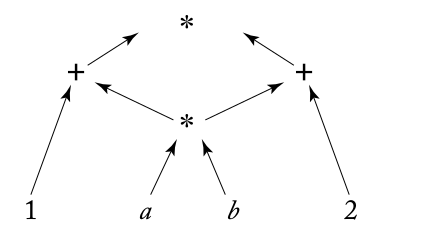
\includegraphics[scale=0.25]{pics/compGraph.png}
\end{figure}

La computación de $a*b$ es compartida. Dado que una red neuronal es esencialmente una expresión matemática, se puede representar como un grafo de cómputo.

La figura anterior muestra el grafo de cómputo para una MLP con una capa oculta y una transformación de salida softmax \cite{goldberg2017neural}. Los nodos ovalados representan operaciones matemáticas o funciones, y los nodos rectangulares sombreados representan parámetros (variables ligadas). Las entradas de la red se tratan como constantes y se dibujan sin un nodo circundante. Los nodos de entrada y parámetros no tienen aristas de entrada, y los nodos de salida no tienen aristas de salida. La salida de cada nodo es una matriz, cuya dimensionalidad se indica sobre el nodo.

Este grafo es incompleto: sin especificar las entradas, no podemos calcular una salida. La figura 5.1b muestra un grafo completo para una MLP que toma tres palabras como entradas y predice la distribución de etiquetas gramaticales para la tercera palabra. Este grafo se puede utilizar para la predicción, pero no para el entrenamiento, ya que la salida es un vector (no un escalar) y el grafo no tiene en cuenta la respuesta correcta ni el término de pérdida. Finalmente, el grafo en la figura 5.1c muestra el grafo de cómputo para un ejemplo de entrenamiento específico, en el cual las entradas son las (incrustaciones de) las palabras "the", "black", "dog", y la salida esperada es "NOUN" (cuyo índice es 5). El nodo de selección implementa una operación de indexación, recibiendo un vector y un índice (en este caso, 5) y devolviendo la entrada correspondiente en el vector.

\subsection{Cómputo hacia Adelante}
El paso hacia adelante (forward pass) calcula las salidas de los nodos en el grafo. Dado que la salida de cada nodo depende únicamente de sí mismo y de las aristas entrantes, es trivial calcular las salidas de todos los nodos.

Esto se hace recorriendo los nodos en un orden topológico y calculando la salida de cada nodo dado que las salidas de sus predecesores ya han sido calculadas.

Más formalmente, en un grafo de $N$ nodos, asociamos a cada nodo un índice $i$ de acuerdo con su orden topológico. Sea $f_i$ la función calculada por el nodo $i$ (por ejemplo, multiplicación, suma, etc.). Sea $\pi(i)$ los nodos padres del nodo $i$, y $\pi^{-1}(i) = \{j | i \in \pi(j)\}$ los nodos hijos del nodo $i$ (estos son los argumentos de $f_i$). Denotemos por $v(i)$ la salida del nodo $i$, es decir, la aplicación de $f_i$ a los valores de salida de sus argumentos $\pi^{-1}(i)$. Para los nodos de variables e entrada, $f_i$ es una función constante y $\pi^{-1}(i)$ está vacío. El paso hacia adelante en el grafo de cómputo calcula los valores $v(i)$ para todos los $i \in [1,N]$.

\begin{figure}[htb]
	\centering
	 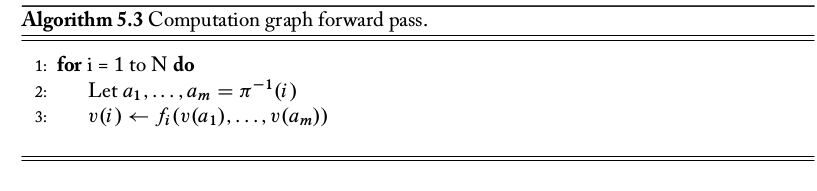
\includegraphics[scale=0.35]{pics/forwardPass.png}
\end{figure}

\subsection{Cómputo hacia Atrás (Retropropagación)}
El paso hacia atrás (backward pass) comienza designando un nodo $N$ con una salida escalar $(1 \times 1)$ como nodo de pérdida y ejecutando el cómputo hacia adelante hasta ese nodo.

El cómputo hacia atrás calcula los gradientes de los parámetros con respecto al valor de ese nodo.

Denotemos por $d(i)$ la cantidad $\frac{\partial N}{\partial i}$. El algoritmo de retropropagación se utiliza para calcular los valores $d(i)$ para todos los nodos $i$.

El paso hacia atrás llena una tabla de valores $d(1), \dots, d(N)$ como se muestra en el siguiente algoritmo.

\begin{figure}[htb]
	\centering
	 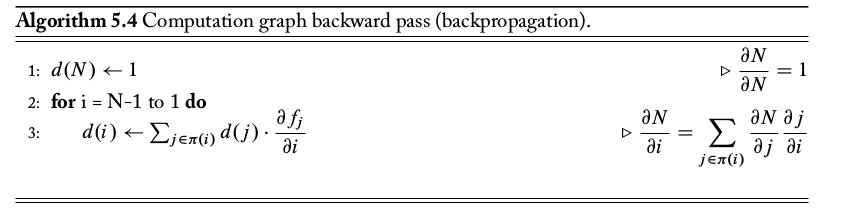
\includegraphics[scale=0.35]{pics/backwardPass.png}
\end{figure}

El algoritmo de retropropagación sigue esencialmente la regla de la cadena de la diferenciación. La cantidad $\frac{\partial f_j}{\partial i}$ es la derivada parcial de $f_j(\pi^{-1}(j))$ con respecto al argumento $i \in \pi^{-1}(j)$. Este valor depende de la función $f_j$ y los valores $v(a_1), \dots, v(a_m)$ (donde $a_1, \dots, a_m = \pi^{-1}(j)$) de sus argumentos, los cuales fueron calculados en el paso hacia adelante.

Por lo tanto, para definir un nuevo tipo de nodo, es necesario definir dos métodos: uno para calcular el valor hacia adelante $v(i)$ basado en las entradas del nodo, y otro para calcular $\frac{\partial f_j}{\partial i}$ para cada $x \in \pi^{-1}(i)$.

\subsection{Resumen de la Abstracción del Grafo de Cómputo}
Observa que la formulación anterior de la retropropagación es equivalente a la dada anteriormente en clase.

La abstracción del grafo de cómputo nos permite:

\begin{enumerate}
  \item Construir fácilmente redes arbitrarias.
  \item Evaluar sus predicciones para entradas dadas (paso hacia adelante).
  \item Calcular gradientes para sus parámetros con respecto a pérdidas escalares arbitrarias (paso hacia atrás o retropropagación).
\end{enumerate}

Una propiedad interesante de la abstracción del grafo de cómputo es que nos permite calcular los gradientes para redes arbitrarias (por ejemplo, redes con conexiones saltadas, pesos compartidos, funciones de pérdida especiales, etc.).

\footnotetext{Un tutorial completo sobre el algoritmo de retropropagación sobre la abstracción del grafo de cómputo se puede encontrar aquí: \url{https://colah.github.io/posts/2015-08-Backprop/}.}

\subsection{Derivadas de funciones no matemáticas}
Definir $\frac{\partial f_j}{\partial i}$ para funciones matemáticas como $log$ o $+$ es sencillo.

Puede resultar desafiante pensar en la derivada de operaciones como pick($\vec{x},5$), que selecciona el quinto elemento de un vector.

La respuesta es pensar en términos de la contribución al cálculo. Después de seleccionar el elemento $i$-ésimo de un vector, solo ese elemento participa en el resto del cálculo.

Por lo tanto, el gradiente de pick($\vec{x},5$) es un vector $\vec{v}$ con la dimensionalidad de $\vec{x}$ donde $\vec{v}_{[5]} = 1$ y $\vec{v}_{[i \neq 5]} = 0$.

De manera similar, para la función $\max(0,x)$, el valor del gradiente es $1$ para $x > 0$ y $0$ en caso contrario.

\section{Regularización y Dropout}
Las redes de múltiples capas pueden ser grandes y tener muchos parámetros, lo que las hace especialmente propensas al sobreajuste.

La regularización del modelo es tan importante en las redes neuronales profundas como lo es en los modelos lineales, tal vez incluso más.

Las regularizaciones discutidas para modelos lineales, es decir, $L_2$, $L_1$ y la elastic-net, también son relevantes para las redes neuronales.

Otra técnica efectiva para evitar que las redes neuronales sobreajusten los datos de entrenamiento es el \textbf{dropout training} \cite{srivastava2014dropout}.

El método de dropout está diseñado para evitar que la red aprenda a depender de unidades o conexiones específicas en el proceso de entrenamiento, lo que ayuda a reducir el sobreajuste.

La idea básica detrás del dropout es apagar aleatoriamente unidades (neuronas) en cada paso de entrenamiento, lo que hace que la red aprenda a ser más robusta y generalice mejor.

El dropout  se puede aplicar a las unidades ocultas (neuronas) y/o a las conexiones entre ellas.

Durante el entrenamiento, en cada paso, se aplica una máscara binaria aleatoria a las unidades o conexiones seleccionadas para el dropout. Las unidades o conexiones que están "apagadas" tienen un valor de cero y no contribuyen al cálculo hacia adelante ni hacia atrás. Solo las unidades o conexiones "encendidas" se utilizan en el cálculo de la predicción y en la retropropagación del error.

Durante la inferencia o evaluación, no se aplica el dropout y todas las unidades o conexiones se utilizan para realizar la predicción.

Es importante destacar que el dropout no es una técnica exclusiva de las redes neuronales, pero ha demostrado ser especialmente efectiva en este contexto debido a la gran cantidad de parámetros y conexiones que suelen tener las redes neuronales profundas.

El valor típico para la tasa de dropout, es decir, la fracción de unidades o conexiones que se apagan en cada paso de entrenamiento, suele ser del orden del 0.2 al 0.5. Sin embargo, el valor óptimo puede variar según el problema y la arquitectura de la red. Por lo tanto, es recomendable experimentar con diferentes tasas de dropout para encontrar la mejor configuración para cada caso.

En resumen, la regularización y el dropout son técnicas efectivas para evitar el sobreajuste en las redes neuronales. Al utilizar regularización, como $L_2$ o $L_1$, se penalizan los grandes valores de los parámetros, lo que ayuda a controlar la complejidad del modelo. El dropout, por otro lado, apaga aleatoriamente unidades o conexiones durante el entrenamiento, lo que promueve la robustez y generalización del modelo. Ambas técnicas pueden utilizarse en conjunto para obtener mejores resultados en la generalización y evitar el sobreajuste.


%Translate this Latex book chapter to Spanish. Output in Latex format. Rearrange bullet points (\items) into full paragraphs. Make sure that sentences are connected in a more fluid way as they come.

\section{Frameworks de Aprendizaje Profundo}
Existen varios paquetes de software que implementan el modelo de grafo de cómputo. Todos estos paquetes admiten todos los componentes esenciales (tipos de nodos) para definir una amplia gama de arquitecturas de redes neuronales.

Uno de estos paquetes es \textbf{TensorFlow} (\url{https://www.tensorflow.org/}), una biblioteca de software de código abierto para cálculos numéricos utilizando gráficos de flujo de datos, desarrollada originalmente por el equipo de Google Brain.

Otro paquete popular es \textbf{Keras}, que es una API de alto nivel para redes neuronales que se ejecuta sobre TensorFlow y otros backends (\url{https://keras.io/}).

También tenemos \textbf{PyTorch}, una biblioteca de aprendizaje automático de código abierto para Python basada en Torch, desarrollada por el grupo de investigación de inteligencia artificial de Facebook. PyTorch admite la construcción de gráficos dinámicos, lo que significa que se crea un grafo de cómputo diferente desde cero para cada muestra de entrenamiento (\url{https://pytorch.org/}).
